\begin{document}
	\chapter{Background}
		The Bitcoin blockchain makes its first appearance in 2008, in an white paper written by someone under the pseudonym of Satoshi Nakamoto \cite{Nakamoto2008} and published on the Cypherpunks mailing list in what is described as "A purely peer-to-peer version of electronic cash that would allow online payments to be sent directly from one party to another without going through a financial institution". In his paper, Nakamoto addresses the problem of the trust-based transaction processors. In his work, Nakamoto asserts that the need of third party in electronic payments brings inherent weaknesses:
		\begin{itemize}
			\item There is no possibility of completely non-reversibile transactions (financial institutes cannot avoid to mediating disputes).
			\item The cost of mediation increases the transaction costs, thus making it impossible for small casual transactions to be processed.
			\item A system that can revert the state of a transactions needs to be trusted. For this reason, merchants tends to ask for customer information, something that doesn't happen with fiat currency.
		\end{itemize}
		Nakamoto suggestion is a peer-to-peer electronic cash system based on the concept of \textit{proof} instead of \textit{trust}: his idea is to make transactions that are computationally impractical to reverse along with a peer-to-peer distributed timestamp service to generate the computational proof of the chronological order the transactions. The other claim Nakamoto does on his paper is that such a system is resilient to attacks as long as the honest nodes of the peer-to-peer network control more computational power than any other cooperating group of attacker nodes, implicitly saying that the system is tolerant to Byzantine failures \cite{Lamport1982}.
		
	\section{Bitcoin Transactions}
		Nakamoto defines the peer-to-peer electronic cash system as a chain of digital transactions where each owner transfers the coin to the next by signing (digitally, in a cryptographic sense) the hash of the previous transactions and the public key of the receiver. The receiver can then verify the signatures to ensure that the chain of ownership was legal. 
		
		\begin{figure}
			\caption{The transaction scheme shows the change of ownership}
			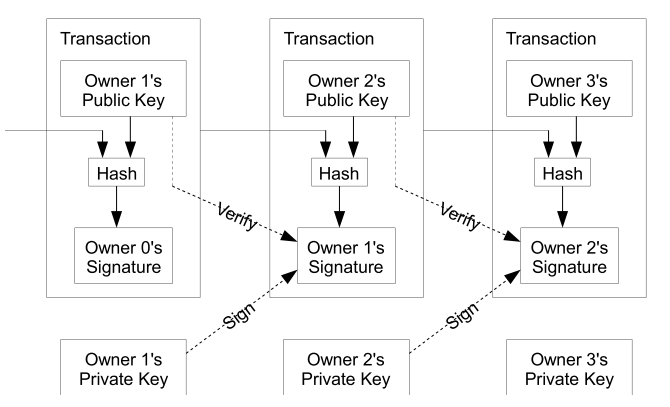
\includegraphics[width=10cm]{transactions.png}
			\centering	
		\end{figure}
	
		The only problem here is that the payee can't prove that the amount the previous owner passed to it was double-spent before the change of ownership. That is, without the full-knowledge of the chronological order of the transactions, a malicious attacker can effectively reuse its money before the payee is able to use it. 
		
		What is needed then is some sort of timestamp service that could put guarantees over the chronological order of the transactions. This is the \textit{trust} that a third party electronic cash system requires to work and what such system does is essentially to check that there exists one and only transaction from the sender to the receiver. Furthermore, this means that a system is required to have the \textit{full-knowledge} of its history, meaning that a decentralized system has as a requirement an \textit{agreement} over a single full history of the transactions. Each transaction must be broadcasted among all the nodes of the network.
		
	\section{Bitcoin Blockchain}
		The solution that Bitcoin (and the majority of the other cryptocurrencies) adopted to provide the full history of the Bitcoin transaction is to store every user's transaction informations on a public ledger replicated among all the nodes of the network. These information are collected in blocks of transactions and each block refers to its predecessor by including its hash.
		
		\begin{figure}
			\caption{Sketch that shows how the blocks refers with their respective predecessor.}
			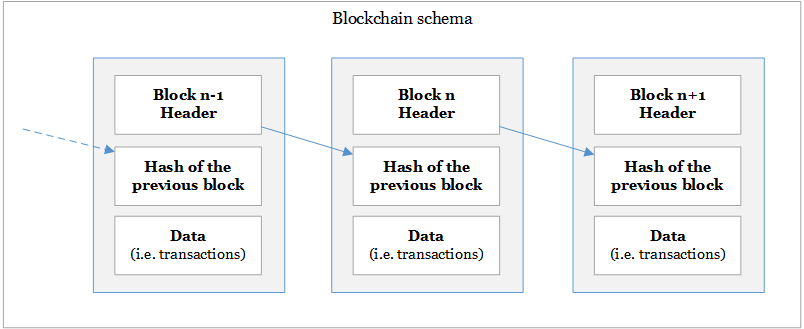
\includegraphics[width=10cm]{blockchain_schema.png}
			\centering	
		\end{figure}
	
		In 2013 C. Decker and R. Wattenhofer \cite{Decker2013} analyzed the behavior of the information propagation in the Bitcoin network and found that the median time for a broadcasted block to reach all the peers is 6.5 seconds (whereas the mean is 12.6 seconds).
		
		What is required then is that the users must all agree on the very same public ledger in order to be sure that a transaction has not been double-spent.
		
	\section{Consensus Mechanism}
		The core innovation and the success of the blockchain technology resides in the consensus protocol which will be referred as \textit{Nakamoto Consensus}. Nakamoto Consensus main goal is to reach an agreement over the same public ledger owned by every node of the network, i.e. old blocks and new blocks must be the same for everyone.
		
		The trick here is to use a challenging computational puzzle (that Nakamoto in his paper calls \textit{Proof-of-work}, but it's a misnomer\footnote{Bitcoin's PoW is not a real Proof of Work because it's a probabilistic puzzle, i.e. with a certain luck one is capable to find a solution with very little work. The very first Proof of Work was invented in 1992 by C. Dwork and M. Naor as an anti-spam system \cite{Dwork1992}}) to determine the next block in the chain. Every user can work on the puzzle and try their luck to get the possibility to find a new block.
		
		A block is appended to the head of the blockchain if and only if it is the first to get announced and contains the correct solution to the computational puzzle. Upon hearing the new block, the participant of the network verify that the block is indeed correct, append the block to the head of their blockchain (that is stored locally) and immediately start working on finding the next one.
		
		The computational puzzle is only needed for all nodes to agree on a common value. Because of its random nature, it is likely that only one node will eventually find the solution to such puzzle. Once a block is found, it is propagated through the network. If the solution to the hashing puzzle is valid and if the transactions in the blocks are valid then the block is accepted into the blockchain. A transaction is valid if:
		\begin{enumerate}
			\item each transaction input matches a previous transaction output.
			\item they are reedemed by their legitimate owners
			\item the sum of values of all transaction outputs is less than or equal to the sum of the values of all inputs.
		\end{enumerate}		
		This verification is performed by bitcoin nodes. It would be useless for a malicious user to forge invalid blocks, because any invalid block (malformed blocks, blocks that contain invalid transactions or blocks whose proof-of-work doesn't resolve the puzzle) would be discarded by the honest peers of the network.
		
		It is possible though that two proof-of-work are found within a short time window. This situation is known as a \textit{temporary fork}, a situation in which the blockchain is split in two chains of equal size and was found to happen with a rate of 1,69 every 100 blocks (\(r = 1,69\%\)) (C. Decker, R. Wattenhofer, 2013). Miners will start to produce a block for either one of the two temporary heads of the chain; the random nature of the computational puzzle will eventually extend one of the two forks and sooner or later every node in the network will reach agreement over the longest chain. Resolving a fork is a crucial matter as forks enable a disruptive attack on the network known as \textit{selfish mining} which reduces the computational powers requirements for attackers from 50\% of the total computational power to 33\% \cite{Eyal2013}. 
		
		Although a fork condition happens not so often, it is always advised to wait at least 6 confirmation blocks (roughly one hour) before considering a transaction to be valid.
		
		\subsection{Producing a block}
		
		A node who decides to actively participate by creating new blocks is called \textit{miner}. What a miner does is to gather the maximum number of transactions that can fit in a block (whose size is fixed) and to find a value (\textit{nonce}) that hash the block and in the meantime whose hash is lesser than a target. More precisely, in order for a block to be valid, the SHA-256 hash of a block's header must be lower to the current \textit{target}, with this last one being a 256-bit number that all the Bitcoin clients share. Finding a block is a cryptographic puzzle, a simple brute force attack on the SHA-256 protocol, whose goal, by picking nonces at random, is to find a hash with \(d\) consecutive zero bits, where \(d\) is called \textit{difficulty} and is derived from the target value in the following way:
		
		\newpage
	
		\[ d = 8 + \frac{log(D)}{16}\] 
		where
		\[D = \frac{\text{max difficulty}}{\text{target}}\]
		
		The difficulty is calibrated every 2016 blocks (roughly two weeks) so that each solution takes approximately 10 minutes to be found. 
		
		The mining operation requires a lot of computational power and the computational power requires a lot of electrical energy, which in 2014 D. Malone and  K.J. O'Dwyer estimated to be comparable to Ireland's electricity consumption \cite{Malone2014}. That is, producing a block has a high production cost associated. To incentivize the production of new blocks, there's a reward for each miner that can be obtained if and only if a block is successfully added to the blockchain: in fact, miners can include a \textit{coinbase} transaction which is capable to generate new coins for the creator of the block; furthermore, this is the only way in which new Bitcoins are input onto the network.
		
		The incentive also protects the system from attackers: suppose an attacker is able to assemble the majority of the computational power, then he would have to choose between using this power to enable a double-spend attack or to generate new coins. It is much more profitable for him to behave good and play by the rules than to destroy the currency.
		
		\section{Ownership}
		
		There is no concept of "account" in Bitcoin. \textit{Ownership} of the currency means knowledge of the private key that is capable to redeem a certain output.
		
		Each transaction output has a signature validation routine (a script) that verify the ownership for those that will claim it. This routine is called \textit{scriptPubKey}, also known as "pay-to-pub-key-hash". It is a script written in the Bitcoin scripting language, a Forth-like, stack language that includes several built-in operations called \textit{opcodes}. 
		
		ECDSA is the protocol used by the Bitcoin network to provide a pair of private and public keys. Every Bitcoin address is the result of the hash of the public portion of the ECDSA private/public key. The amount of Bitcoins that reside in an address can be spent only if a user can prove with his signature that he is the owner of the Bitcoin address. To redeem the coins of an address, the owner proves his identity by inputting the signature and the public key of the \textit{scriptSig} to a \textit{scriptPubKey} of a previous transaction.
		
		\newpage
		
		Given the following \textit{scriptSig} and \textit{scriptPubKey}:
		\begin{verbatim}
		scriptPubKey: OP_DUP OP_HASH160 <pubKeyHash> OP_EQUALVERIFY OP_CHECKSIG
		scriptSig: <sig> <pubKey>
		\end{verbatim}
		
		The validation \footnote{from the Bitcoin wiki. https://en.bitcoin.it/wiki/Transaction\#Pay-to-PubkeyHash}:
		\begin{center}
			\begin{tabulary}{\textwidth}{|L|C|L|}
			\hline
			\textbf{Stack} & \textbf{Script} & \textbf{Description} \\ \hline
			Empty. & <sig><pubKey> OP\_DUP OP\_HASH160 <pubKeyHash> OP\_EQUALVERIFY OP\_CHECKSIG & scriptSig and scriptPubKey are combined. \\ \hline
			<sig> <pubKey> & OP\_DUP OP\_HASH160 <pubKeyHash> OP\_EQUALVERIFY OP\_CHECKSIG & Constants are added to the stack. \\ \hline
			<sig> <pubKey> <pubKey> & OP\_HASH160 <pubKeyHash> OP\_EQUALVERIFY OP\_CHECKSIG & Top stack item is duplicated. \\ \hline
			<sig> <pubKey> <pubHashA> & <pubKeyHash> OP\_EQUALVERIFY OP\_CHECKSIG & Top stack item is hashed. \\ \hline
			<sig> <pubKey> <pubHashA> <pubKeyHash> & OP\_EQUALVERIFY OP\_CHECKSIG & Constant added. \\ \hline
			<sig> <pubKey> & OP\_CHECKSIG & Equality is checked between the top two stack items. \\ \hline
			true & Empty. & Signature is checked for top two stack items. \\
			\hline
			\end{tabulary}
		\end{center}
		
	\end{document}